\documentclass[12pt]{article} % Here we state, that we need the text size to be 12p and we want article setup

\usepackage[utf8]{inputenc} % Allows the user to input accented characters directly from the keyboard
\usepackage[T1]{fontenc} % Oriented to output, that is, what fonts to use for printing characters
\usepackage[english]{babel} % The language, you are writing in - you should be able to change to danish

\usepackage[margin=2.5cm]{geometry} % How big margins we want
\geometry{a4paper} % What type of paper we want

\setlength\parindent{0pt} % Makes \noindent standard (my preference - not everyones!)

\usepackage{todonotes} % With this, you can add todo-notes: \todo{stuff todo} or \todo[inline]{stuff todo}
\usepackage{caption} % You can create captions for your tables, pictures etc. AND YOU WANT TO DO THAT
\usepackage{wrapfig} % Allows in-line images if needed
\usepackage{hyperref} % Allows you to create hyperlinks within the document
\hypersetup{colorlinks=false,hidelinks, citecolor=black, urlcolor=black}
\usepackage{url} % Enables typesetting of hyperlinks

\usepackage{amsmath} % Math in your tex 
\usepackage{amsfonts} % Math in your tex 
\usepackage{mathtools} % Math in your tex 
\DeclarePairedDelimiter{\ceil}{\lceil}{\rceil} % Math in your tex 

\usepackage{csquotes} % Provides advanced facilities for inline and display quotations
\usepackage[titletoc]{appendix} % Names appendices "Appendix A" instead of just A in Contents

\usepackage{pdfpages} % We can now import pdf files to our tex file - win!
\usepackage{graphicx} % We can now import pictures - uhlalalah!

\usepackage{algorithm} % http://ctan.org/pkg/algorithms
\usepackage{algpseudocode} % http://ctan.org/pkg/algorithmicx
\usepackage{listings}
\usepackage{color}
\usepackage{graphicx}
\usepackage{lipsum}
\usepackage{cleveref}

\definecolor{bluekeywords}{rgb}{0.13,0.13,1}
\definecolor{greencomments}{rgb}{0,0.5,0}
\definecolor{turqusnumbers}{rgb}{0.17,0.57,0.69}
\definecolor{redstrings}{rgb}{0.5,0,0}

\lstdefinelanguage{FSharp}
                {morekeywords={let, new, match, with, rec, open, module, namespace, type, of, member, and, for, in, do, begin, end, fun, function, try, mutable, if, then, else},
    keywordstyle=\color{bluekeywords},
    sensitive=false,
    morecomment=[l][\color{greencomments}]{///},
    morecomment=[l][\color{greencomments}]{//},
    morecomment=[s][\color{greencomments}]{{(*}{*)}},
    morestring=[b]",
    stringstyle=\color{redstrings}
    }
\graphicspath{ {images/} } 
\usepackage{natbib} % Bibliography stuff


%-----------------------------------------------------------------------------
% HEADER AND FOOTER STUFF
%-----------------------------------------------------------------------------
\usepackage{fancyhdr}
\usepackage{lastpage} % Making it possible to write ``Page x of y'' in the footer

\pagestyle{fancy}
\fancyhf{}
% Header stuff below
\lhead{Mark Roland Larsen} 
\chead{}
\rhead{fvg932} 
% Footer stuff below
\cfoot{Page \thepage \hspace{1pt} of \pageref{LastPage}} % To the left at the bottom

%-----------------------------------------------------------------------------
\begin{document} % You always need this


\includepdf[pages={-}]{forside.pdf} % How we get our fancy frontpage imported to our file


%-----------------------------------------------------------------------------
% ABSTRACT STUFF (only needed if you have to write this sort of things ;o) )
%-----------------------------------------------------------------------------

%\begin{abstract}
%\noindent 
%\end{abstract}

%-----------------------------------------------------------------------------
% CONTENT STUFF
%-----------------------------------------------------------------------------

\newpage % I want my table of contents on its own page
\tableofcontents
\newpage

%\renewcommand{\abstractname}{Acknowledgements} % If you want to thank someone, this is the way 
%\begin{abstract}
%\noindent 
%\end{abstract}



%-----------------------------------------------------------------------------
% ACTUAL CONTENT STUFF
%-----------------------------------------------------------------------------

\section{Abstract}

\section{Description}

\section{Preface}

\section{Limitations}

I følgende opgave arbejdes der på binære træer med typen 

\section{Introduction}

The string matching problem is found in various fields of study \cite{mit}. In biology, string matching algorithms significantly aid biologists in retrieving and comparing DNA strings, reconstructing DNA strings from overlapping string fragments and looking for new or presented patterns occurring in a DNA\cite{gusfield}. Text-editing applications also adopt string matching algorithms, whenever the application has to acquire an unambiguous occurrences of a user-given pattern, such as a word in some document\cite{introduction, gusfield}. String matching is used in music equipment, AI (artificial intelligence) and in addition, various software applications like virus scanners (anti-virus) or intrusion detection systems, frequently adopt string matching algorithms as a practical tool, to secure data security over the internet \cite{detection}.
Fundamentally, string matching is a method to find some pattern $P =\{p_1,p_2,…,p_n\}$ in a given text $T=\{t_1, t_2,…,t_m\}$, over some finite alphabet $\Sigma$ as illustrated in \cref{fig:banana} \cite{detection}.

\section {String Matching}

String matching is both an algorithmic problem and data structure problem. The static data structure consist of preprocessing some predefined large text $T = \{t_1, t_2, …, t_m}\}$, and query some smaller pattern $P=\{p_1, p_2,...,p_n\}$ \cite{mit}. The objective is to preprocess text $T$ and query pattern $P$ in text $T$ in linear time, $O(m), m \in |T|$ 
\footnote{See \cref{sec:One} for a description of algorithmic time analysis} and $O(n), n \in |P|$, respectively \cite{mit}.  
\newline
Following the tradition of Gusfield et al. this discussion begins with the naive methoed of the exact string matching paradigm.
\newline
\\*
Problem:
\begin{quote}
Given a pattern $P$ and a long text $T$, the problem consist of finding all occurrences of pattern $P$, if any, in text $T$ \cite{gusfield}.
\end{quote}
\newline
The occurrences of pattern $P=\{ana\}$ in text $T=\{banana\}$ are found at $T[1,3]$ and $T[3,5]$, as illustrated in Figure \ref{fig:banana}. Note that pattern $P$ may overlap.
\begin{figure}[h]
    \centering
    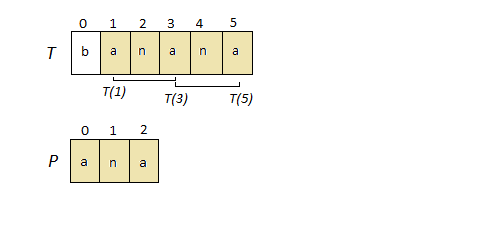
\includegraphics[width=0.6\textwidth]{1}
    \captionsetup{width=0.8\textwidth}
    \caption{The text $T$=\{banana\} and pattern $P$=\{ana\} over the alphabet $\Sigma$=\{abn\}. The pattern $P$ occours in $T$ in, at position $T[1]$ and $T[3]$. Notice that occurrences of $P$ may overlap.}
    \label{fig:banana}
\end{figure}
\newline



\subsection{Suffix trees}

The classic application for suffix tree is the substring problem \cite{gusfield, Kunihiko}, which is both a data structure -and an algorithmic problem \cite{mit}. That is, given a long text $T$ over some alphabet $\Sigma$, and some pattern $P$, the substring problem consist of preprocessing $T$ in linear time $O(m)$, and hereafter  $T$ should be able to take any unknown pattern $P$, and in linear time $O(n)$ determine occurrences of $ P$, if any, in $T$ \cite{gusfield}. The preprocessing time is here proportional to the length of text $T$, and the query is proportional to the length of pattern $P$ \cite{gusfield}. 
\newline
This paper adopts the approach of Gusfield et al., by not applying the denotation of pattern $P$ and text $T$, in respect to describing suffix trees. By using the general description and denotation of suffix trees, there will be less confusion, since input string can take different roles and vary for application to application \cite{gusfield}.
\newline
\newline
Conceptually a suffix tree is a compressed trie \cite{mit}.  
\begin{quote}
\textbf{Definition}    A trie contains all suffixes of string $S$, where each edge is labeled with a character from some alphabet $\Sigma$. Each path from root to leaf represent a suffix, and every suffix is represented with some path from root to leaf \cite{mit,Kunihiko}.
\end{quote}
\begin{figure}[h]
    \centering
    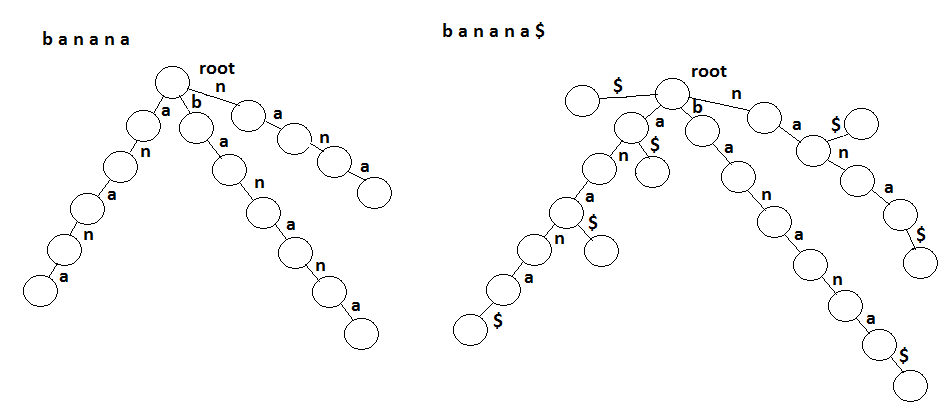
\includegraphics[width=0.6\textwidth]{trie}
    \captionsetup{width=0.8\textwidth}
    \caption{Left is a trie of the string $banana$ and the right is a trie of the string $banana\$$.}
    \label{fig:trie}
\end{figure}
\newline
Figure \ref{fig:trie} illustrates two tries, left of the string banana and the right over the string $banana\$$. Note that right trie has the termination character $\$$ appended to the end. This is due to the fact that the definition of a trie dictates that every suffix is represented with some path from root to leaf. Suffix $ana$ in left trie does not have a path from root to leaf, but appending a termination character to S that exists nowhere else in the string, will eliminate the problem.
\newline
Creating a compressed trie, one takes each non-branching nodes and compress them, such that edge-labels from non-branching nodes concatenates into a new edge-label, as illustrated in Figure \ref{fig:comprestrie}. Here node 1 is a non-branching node, one then concatenate a to n, to form a new edge-label na, deleting the non-branching node \cite{mit}. The number of non-branching nodes in a trie is at most the number of leaves. By compressing, we know have that the number of internal nodes is at most the number of leaves, having O(k) nodes total.
\newline

\begin{figure}[h]
    \centering
    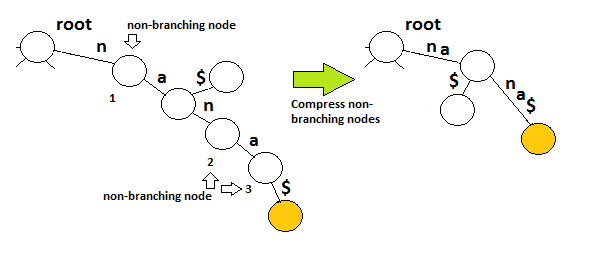
\includegraphics[width=0.6\textwidth]{compressingtrie}
    \captionsetup{width=0.8\textwidth}
    \caption{Compressing a trie.}
    \label{fig:comprestrie}
\end{figure}
\begin{quote}
\textbf{Definition}   A Suffix tree, $T$, is a $m$-character string $S$ concatenated with a termination character $\$$, that is represented as a directed rooted tree with exactly $m$ leaves, numbered $1$ to $m$. Except the root, each internal node contains at least two children, with each edge labeled with a nonempty substring of S. No two edges exiting a node can have labels beginning with the same character. The concatenation of edge-labels on the path from the root to leaf i, unerringly spells out the suffix of $S$ that starts at position i, such that it spells out $S[i..m]$. The termination character $\$$ is assumed to appear nowhere else in $S$, such that no suffix of the consequential string can be a prefix of any other suffix\cite{gusfield}.
\end{quote}
\begin{figure}[h]
    \centering
    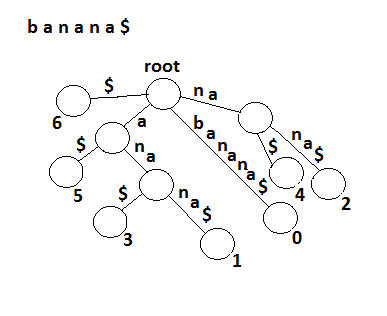
\includegraphics[width=0.4\textwidth]{suffixtree(banana)}
    \captionsetup{width=0.8\textwidth}
    \caption{A suffix tree $T$ for string $banana\$$.}
    \label{fig:suffixTree}
\end{figure}
The suffix tree for the string $banana\$$, in lexicographical order, is illustrated \ref{fig:suffixTree}. Each path from the root to a leaf $i$, unerringly spells out a suffix of $S$, starting at position $i$ in $S$. As an example, leaf numbered $2$ spells out $nana\$$, starting at position $2$ in the $S$, such that $S[2..6] = nana\$$. Each node has at least two children, and no two edges exiting a node begins with the same character. 
\newline
To dive into the substring problem using linear preprocessing time, $O(m)$, and linear search time, $O(n)$ we follow the tradition, and starts with a naive and straightforward algorithm to building suffix trees before verturing into the linear time preprocessing approach \cite{gusfield}. 

\subsection{Knutt-Moris-Pratt Algorithm}

\subsection{Operations on suffix trees}

Bla bla bla...
\newline

\subsubsection{Insertion \& Deletion}
\subsubsection{Lowest Common Ancestor}

An interesting application of suffix trees is the $lca$ (Lowest Common Ancestor) problem, that is, finding the lowest common ancestor of node $i$ and $j$ in tree $T$. 
Lowest common ancestor was first obtained by Harel and Tarjan (1984, published online 2006 \cite{lcaWeb}) and later on simplified by Schieber and Vishkin (1988, published online in 2006 \cite{lcaWebSch})\cite{gusfield}.
\newline
Lowest common ancestor is an interesting application given that it is used in application as exact matching with wild cards and the $k$-mismatch problem, amongst others \cite{gusfield}. More interesting is the fact that $lca$ of leaves $i$ and $j$ identifies the longest common prefix of suffixes $i$ and $j$, which will be discussed later on.
\newline
By consuming linear time amount of preprocessing a suffix tree, that is a rooted tree, any two nodes can be identified and their $lca$ can be found in constant time, $O(1)$ \cite{gusfield, lca}. This paper will not dwell into the different linear time preprocessing algorithms for the $lca$ predicament, but delivers an overview and clarification of the problem by introducing a simpler but slower algorithm. (maybe linear in the appendix?).
\begin{quote}
\textbf{Definition}   In a rooted tree $T$ a node $u$ is an ancestor of node $v$, if $u$ is an unique path from the root to $v$ \cite{gusfield}.
\end{quote}
\begin{quote}
\textbf{Definition}   In a rooted tree $T$, the lowest common ancestor of two node $u$ and $v$, is the deepest node in tree $T$ that is an ancestor of both $u$ and $v$ \cite{gusfield}.
\end{quote}
Let’s suppose for simplification that an application is allowed preprocessing time of an upper bound of $\theta (n lg n)$, which is an acceptable bound for most applications \cite{gusfield}. Then, in the preprocessing state of tree $T$, perform a deept-first traversal of tree $T$ and create a list $L$ of nodes in order as they are visited. Then locating the $lca$ of node $2$ and $8$, $lca[2,8]$, in \cref{fig:travesal}, one only have to find any occurrences of $2$ and $8$ in $L$. Then take the lowest value in interval between $L[1] = 2$ and $L[12]=8$. This value is the lowest common ancestor for node $2$ and $8$ in $T$, $lca[2,8]=1$.
\begin{figure}[h]
    \centering
    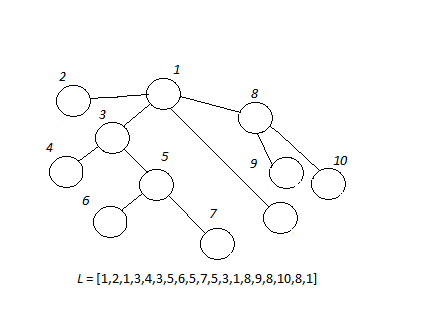
\includegraphics[width=0.5\textwidth]{travesal}
    \captionsetup{width=0.8\textwidth}
    \caption{Rooted tree - deept-first travesal with $L = [1,2,1,3,4,3,5,6,5,7,5,3,1,8,9,8,10,8,1]$}
    \label{fig:travesal}
\end{figure}


\subsubsection{Longest Common Prefix}

\begin{figure}[h]
    \centering
    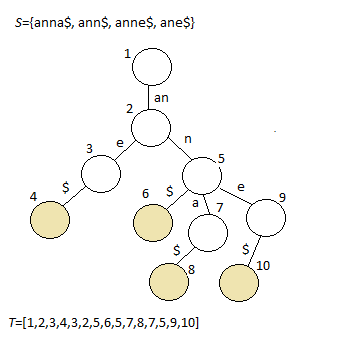
\includegraphics[width=0.4\textwidth]{suffixtree(speeling_anna)}
    \captionsetup{width=0.8\textwidth}
    \caption{Rooted tree - deept-first travesal with $L = [1,2,1,3,4,3,5,6,5,7,5,3,1,8,9,8,10,8,1]$}
    \label{fig:travesal_anna}
\end{figure}

\subsubsection{Predecessor $\&$ successor amongst strings}
\subsubsection{Lowest Common Extension}




\subsection{Suffix arrays}
\subsection{Suffix Array Induced Sorting Algorithm (SA-IS)}
\subsection{SA-IS - correctness and completeness}
\subsection{Operations on suffix arrays}

\section{Malware Detection System - A string matching approach}
\subsection{Understanding Malware}
\subsection{Building database of known malware - SHA1 encryption}
\subsection{String matching in Malware detection systems}
\subsection{Building interactive systems - Windows (R) Forms}
\subsection{Implementing a Malware detection system using preprocessed suffix arrays of known malware}

\section{Evaluation and recommendations}

Jeg har ikke nået at lave denne, men smider alle opgaverne til dig torsdag eller fredag, som jeg skal beskrevet i mailen.
Håber det er iorden.

\section{Discussion}
\cite{gusfield}

\section{Future work}

\section{Conclussion}
\section{Literature list and references}
\section{Appendix}



%-----------------------------------------------------------------------------

%-----------------------------------------------------------------------------
\newpage
\appendix
\label{appendix}
\section{One}\label{sec:One}
\lipsum[21]
%I will let this talk for it self. And no, you don't need it right now, so out comment it or delete it $\ddot\smile$


% THIS I WILL NOT EXPLAIN RIGHT NOW - WE CAN TAKE IT WHEN IT IS MORE RELEVANT!
\newpage
\nocite{*}
\bibliographystyle{ieeetr}
\bibliographystyle{unsrt}
\bibliography{bibliography}
%-----------------------------------------------------------------------------
\end{document}